To gain a better understanding of the areas in which the models are struggling, we will conduct a qualitative analysis of failure cases from the test set.
We focus on examples with significant orientation errors, particularly those around \qty{90}{\degree} and \qty{180}{\degree}, as these are indicative of challenging scenarios or annotation issues.

\Cref{fig:failure_modes} shows three representative failure examples per model, grouped by error type.
The top row illustrates the worst orientation errors, while the bottom row shows examples with errors around \qty{90}{\degree}.
Each panel displays the input image, the ground-truth mask, the predicted mask and the measured orientation error.

For \qty{180}{\degree} errors, the majority appear to stem from annotation errors rather than model mistakes: in all the examples shown, the annotated head and tail regions are reversed compared to the visible anatomy, while the model predictions point in the correct direction despite the imperfect masks.
For instance, the UNet3 prediction in the first image provides a blurry yet correctly oriented segmentation, whereas the annotation erroneously labels the tail as the head.
Similarly, the ResUNet18 predictions align well with the actual bee orientation, even when the annotation is flipped.

Both models struggle with \qty{90}{\degree} errors in highly cluttered images where no bee is fully visible.
In the UNet3 examples, the predicted masks are diffuse and are often confused by surrounding bees.
The annotations themselves are ambiguous or clearly do not correspond to any individual bee.
ResUNet18 performs better, often correctly segmenting one plausible bee even when the annotation does not correspond to it.
In some cases, the image quality or visibility is so poor that neither the model nor the annotation appears reliable.

These examples highlight the limitations of the models, particularly in cluttered and low-quality regions, as well as the inconsistencies in the ground-truth annotations, which may artificially inflate measured errors.



\begin{figure}[htbp]
    \centering
    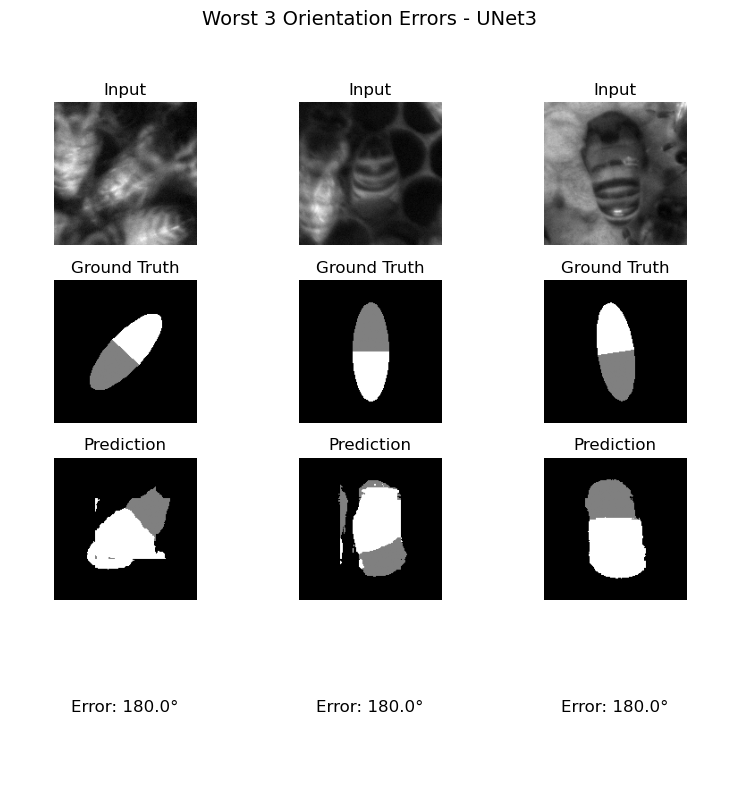
\includegraphics[width=0.49\textwidth]{figures/results/5 - fails/UNet3 Worst Orientation Errors.png}
    \hfill
    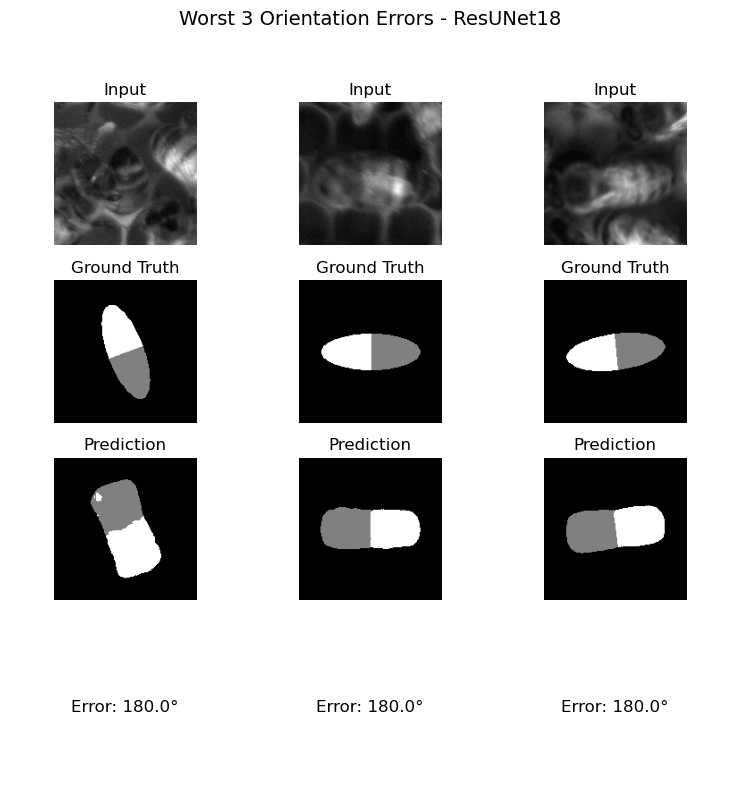
\includegraphics[width=0.49\textwidth]{figures/results/5 - fails/ResUNet18 Worst Orientation Errors.png}

    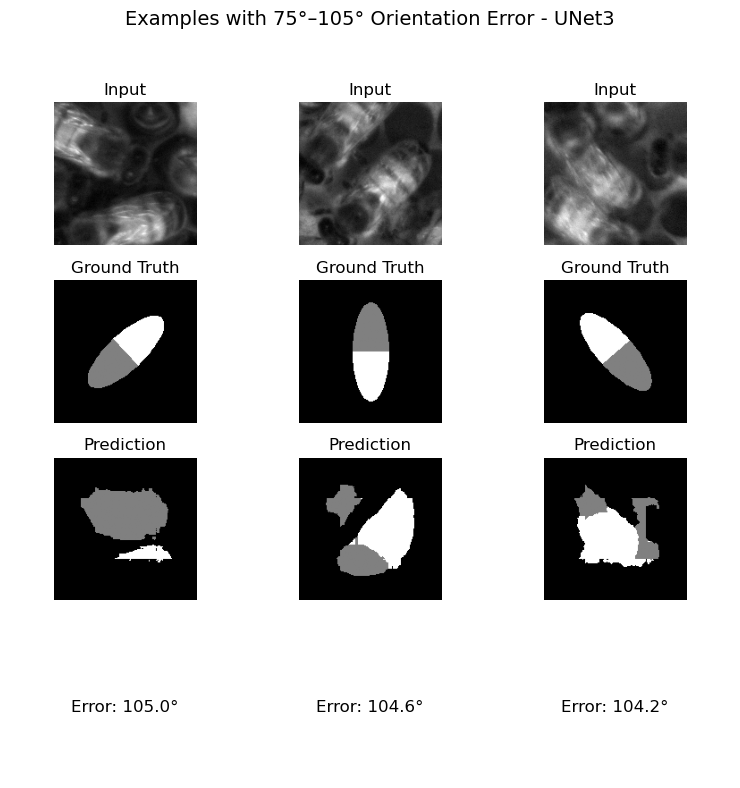
\includegraphics[width=0.49\textwidth]{figures/results/5 - fails/UNet3 Orientation Errors 90deg Range.png}
    \hfill
    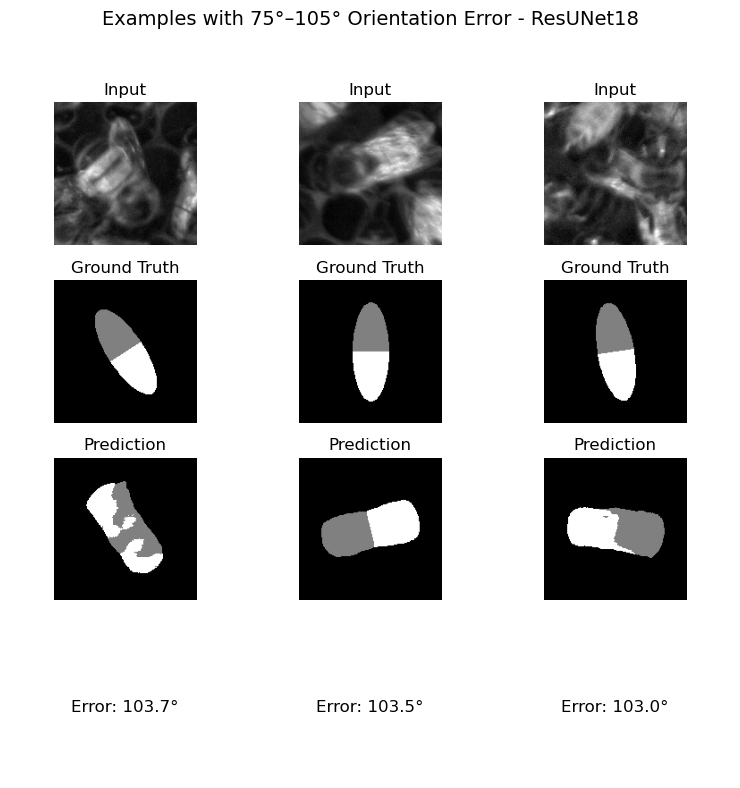
\includegraphics[width=0.49\textwidth]{figures/results/5 - fails/ResUNet18 Orientation Errors 90deg Range.png}
    \caption{
        Qualitative failure cases for UNet3 (\textbf{left}) and ResUNet18 (\textbf{right}), with the worst absolute orientation errors (\textbf{top row}) and examples with errors around \qty{90}{\degree} (\textbf{bottom row}).
        Each panel shows the input image, ground‑truth mask, predicted mask, and measured error.
        In the worst (\qty{180}{\degree}) cases, annotations are often flipped, while model predictions remain plausible.
        Around \qty{90}{\degree}, both models struggle in highly cluttered or ambiguous scenes, but ResUNet18 still produces more coherent segmentations than UNet3.
    }
    \label{fig:failure_modes}
\end{figure}